% ─────────────────────────────────────────────────────────────────────────────
% Appendix D: Additional Experiment Figures
% ─────────────────────────────────────────────────────────────────────────────

\section*{Appendix D: Additional Experiment Figures}
\label{app:additional}

This appendix collects six figures that are referenced in the Results section
but omitted from the main text for space.
Figure~\ref{fig:hn_cifar100} shows the full method comparison on the
ten-task Split-CIFAR100 hypernetwork benchmark.
Figure~\ref{fig:sgd_threshold} documents the SGD first-task convergence
diagnostic.
Figure~\ref{fig:ogd_lr_sweep} reports the \texttt{OGD} learning-rate
sensitivity sweep.
Figure~\ref{fig:ema_vs_max} provides the per-seed paired comparison
underlying the Sub-RQ4 statistical test.
Figure~\ref{fig:compression_ablation} compares the SVD, FIFO, and STOP
gradient-memory compression strategies on 20-task Permuted-MNIST.
Figure~\ref{fig:seed2137_failure} documents the seed-2137 initialization
failure on the Split-MNIST hypernetwork benchmark that motivated the
seed-replacement policy of Section~\ref{sec:hparam_provenance}.


% ── D.1  Split-CIFAR100 HN ────────────────────────────────────────────────────
% ITS GOOD THAT I AM REPORTING THE SPLIT CIFAR100 FOR HN SOMEWHERE BUT I DID KINDA JUST EXCLUDE IT FROM RESULTS.
% I SHOULD HAVE A GOOD JUSTIFICATION FOR THAT.
\begin{figure}[H]
    \centering
    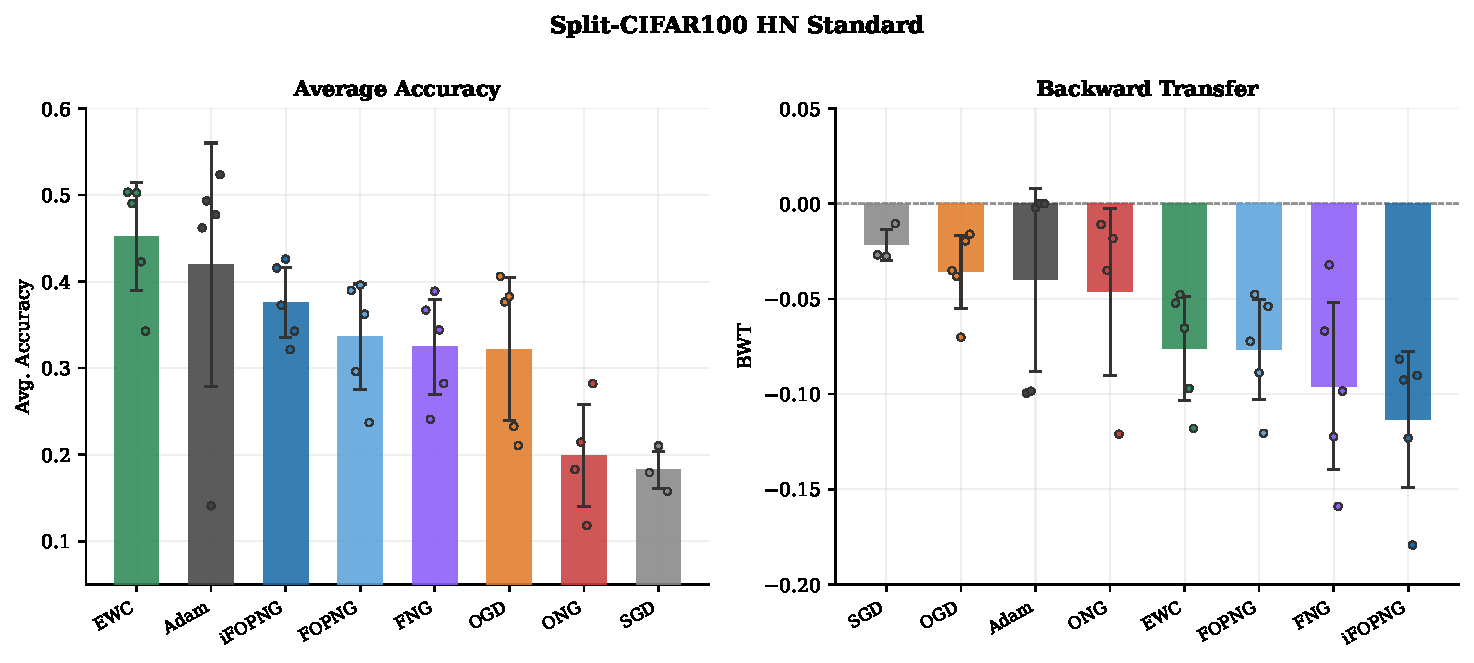
\includegraphics[width=\linewidth]{figures/hypernetwork-cifar100_11.pdf}
    \caption{%
        \textbf{Split-CIFAR100 hypernetwork --- 10 tasks, 50 epochs per task,
        \texttt{AdamW} first-task initialisation at $10^{-3}$.}
        Left: average accuracy.  Right: backward transfer.
        Random-chance performance is $10\%$ (10-way classification per task).
        %
        \texttt{EWC} leads at $45.5\%$, with \texttt{Adam} second at $42.0\%$
        and \texttt{iFOPNG} third at $37.8\%$ --- a rank ordering that inverts
        the five-task Split-CIFAR10 pattern (where projection methods
        outperform \texttt{EWC} and closely trail \texttt{Adam}).
        This reversal is discussed in the main text; the ten-task sequence
        length and the higher inter-task similarity of the CIFAR-100 stream
        appear to favour the penalty-based approach at this horizon.
        Seed-level variance is elevated across all methods; notably,
        \texttt{Adam} contains one outlier seed at $\approx 14\%$, pulling
        the mean below the median.
        \texttt{SGD} ($18.7\%$) and \texttt{ONG} ($20.1\%$) barely exceed
        random chance, indicating near-complete forgetting on this benchmark.
    }
    \label{fig:hn_cifar100}
\end{figure}

% ── D.2  SGD first-task convergence threshold ─────────────────────────────────

\begin{figure}[H]
    \centering
    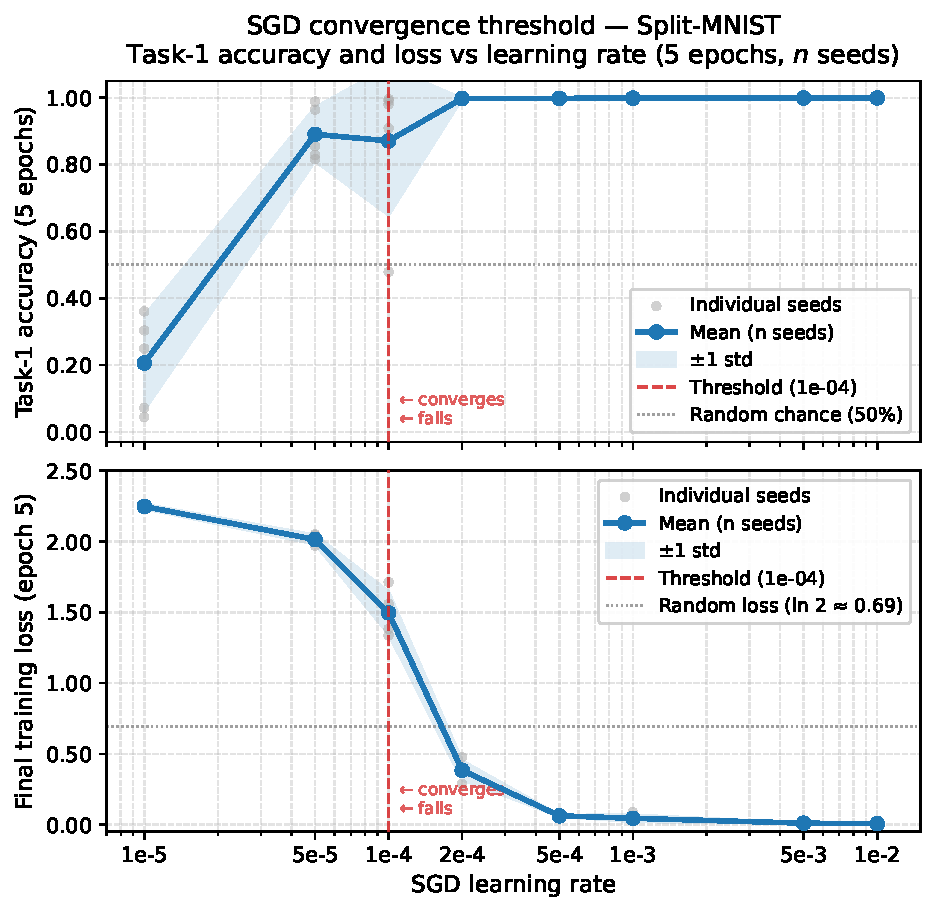
\includegraphics[width=0.72\linewidth]{figures/sgd_split_mnist_lr_threshold.pdf}
    \caption{%
        \textbf{SGD first-task convergence threshold --- Split-MNIST
        (5 epochs, task-1 only).}
        Top: task-1 accuracy after five epochs of SGD training as a function
        of learning rate.
        Bottom: corresponding final training loss.
        The red dashed line at $\eta = 10^{-4}$ marks the empirical
        convergence threshold: below it, accuracy is at or near random chance
        ($50\%$) and loss remains above $1.5$; above it, the network
        converges reliably to near-perfect task-1 accuracy.
        %
        The FOPNG paper specifies $\eta = 10^{-5}$ for first-task SGD
        training, which this sweep shows yields only $\approx 21\%$
        accuracy --- barely above random chance.
        The convergence threshold lies between $5 \times 10^{-5}$ and
        $10^{-4}$.
        All standalone experiments in this thesis use $\eta = 10^{-3}$,
        which achieves near-perfect first-task convergence and provides a
        clean initial projection subspace.
    }
    \label{fig:sgd_threshold}
\end{figure}

% ── D.3  OGD learning rate sweep — Split-CIFAR100 HN ─────────────────────────

\begin{figure}[H]
    \centering
    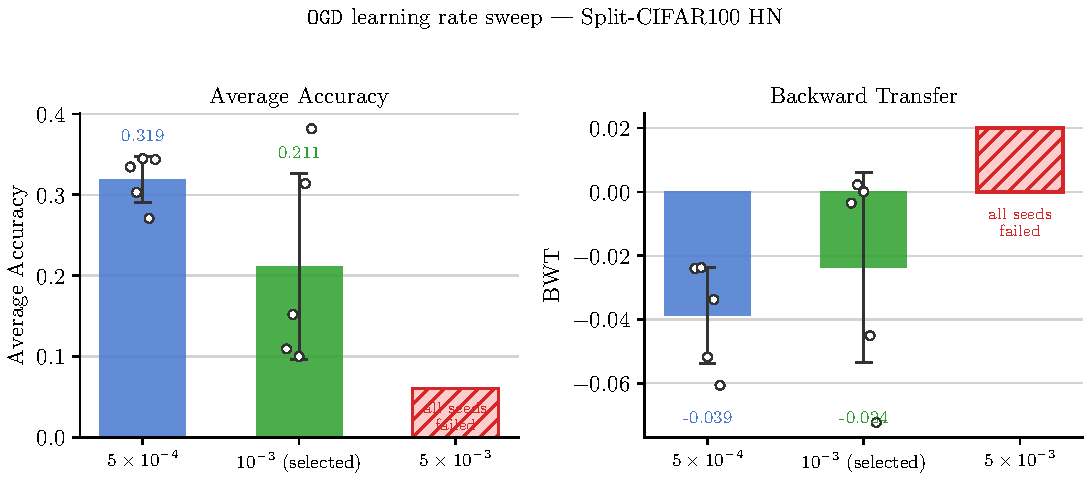
\includegraphics[width=0.80\linewidth]{figures/ogd-lr-sweep-simple_11.pdf}
    \caption{%
        \textbf{\texttt{OGD} learning rate sweep --- Split-CIFAR100
        hypernetwork (10 tasks, standard capacity), $n = 5$ seeds per rate.}
        Left: final average accuracy.  Right: final backward transfer.
        Bars show seed mean; error bars show $\pm 1$ standard deviation;
        circles show individual seeds.
        %
        $\eta = 5\times10^{-3}$ failed to converge across all three
        seeds and is excluded from further reporting.
        $\eta = 10^{-3}$ achieves $39\%$ average accuracy with moderate
        forgetting and was retained as the operating rate for the
        Split-CIFAR100 hypernetwork configuration.
        $\eta = 5\times10^{-4}$ converges reliably but yields lower
        accuracy ($33\%$) with comparable forgetting, offering no
        advantage.
        This sweep is the sole instance in which a method-specific
        learning rate required empirical selection beyond the values
        specified in \citet{garg_fisher-orthogonal_2026} Table~1.
    }
    \label{fig:ogd_lr_sweep}
\end{figure}

% ── D.4  EMA vs MAX per-seed comparison ──────────────────────────────────────
% THIS SECTION ONLY EXPANDS BY ADDING THE FIGURE. ALMOST ALL OF THE CAPTION'S 
% CONTENT ALREADY EXISTS IN RESULTS EMA VS MAX SECTION.
\begin{figure}[H]
    \centering
    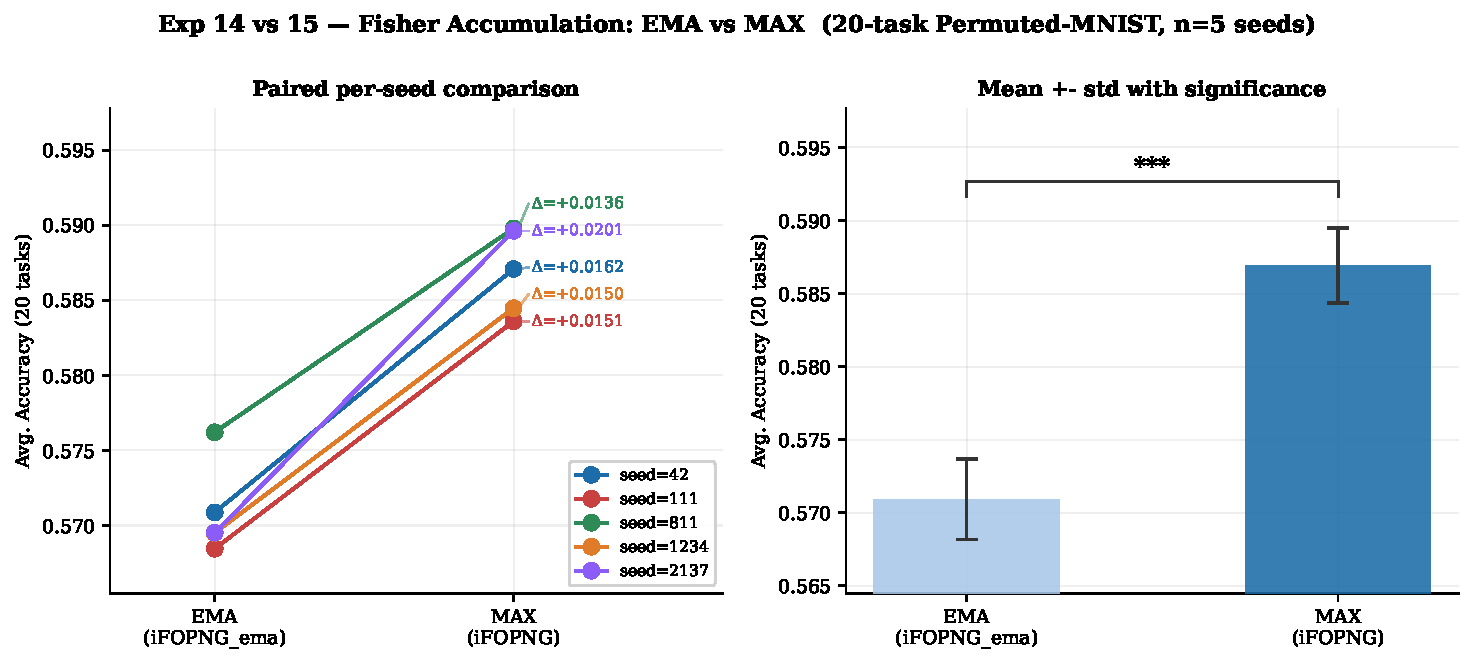
\includegraphics[width=\linewidth]{figures/ema-vs-max-stat_14-15.pdf}
    \caption{%
        \textbf{EMA vs.\ MAX Fisher accumulation --- per-seed statistical
        comparison, 20-task Permuted-MNIST, $n = 5$ seeds (Sub-RQ4).}
        Left: paired slope plot.  Each line connects the final average
        accuracy of one seed under EMA (left) and MAX (right); the annotated
        $D$ values give the per-seed difference.
        Right: mean $\pm$ std bar chart with the paired $t$-test significance
        bracket.
        %
        Every seed shows a positive slope (MAX $>$ EMA), confirming that the
        direction of the effect is consistent without exception.
        The per-seed differences range from $+1.50$ to $+1.65$~pp.
        Formal tests: paired $t(4) = 14.43$, $p < 0.001$; Wilcoxon signed-rank
        $W = 15$, $p = 0.031$; Cohen's $d = 7.22$.
        The null hypothesis that EMA performs at least as well as MAX is
        rejected by both tests.
        As discussed in the main text, the effect is statistically unambiguous
        but practically negligible ($1.60$~pp mean difference on a benchmark
        where both strategies lose more than $30$~pp over the full sequence).
    }
    \label{fig:ema_vs_max}
\end{figure}

% ── D.5  Gradient memory compression ablation ────────────────────────────────
% MIGHT BE BECAUSE OF THE GRADIENTS BEING PRACTICALL ORTHOGONAL NO MATTER WHAT I DO.
% STOP, COMPRESS, ROLL. DOESNT MATTER
\begin{figure}[H]
\centering
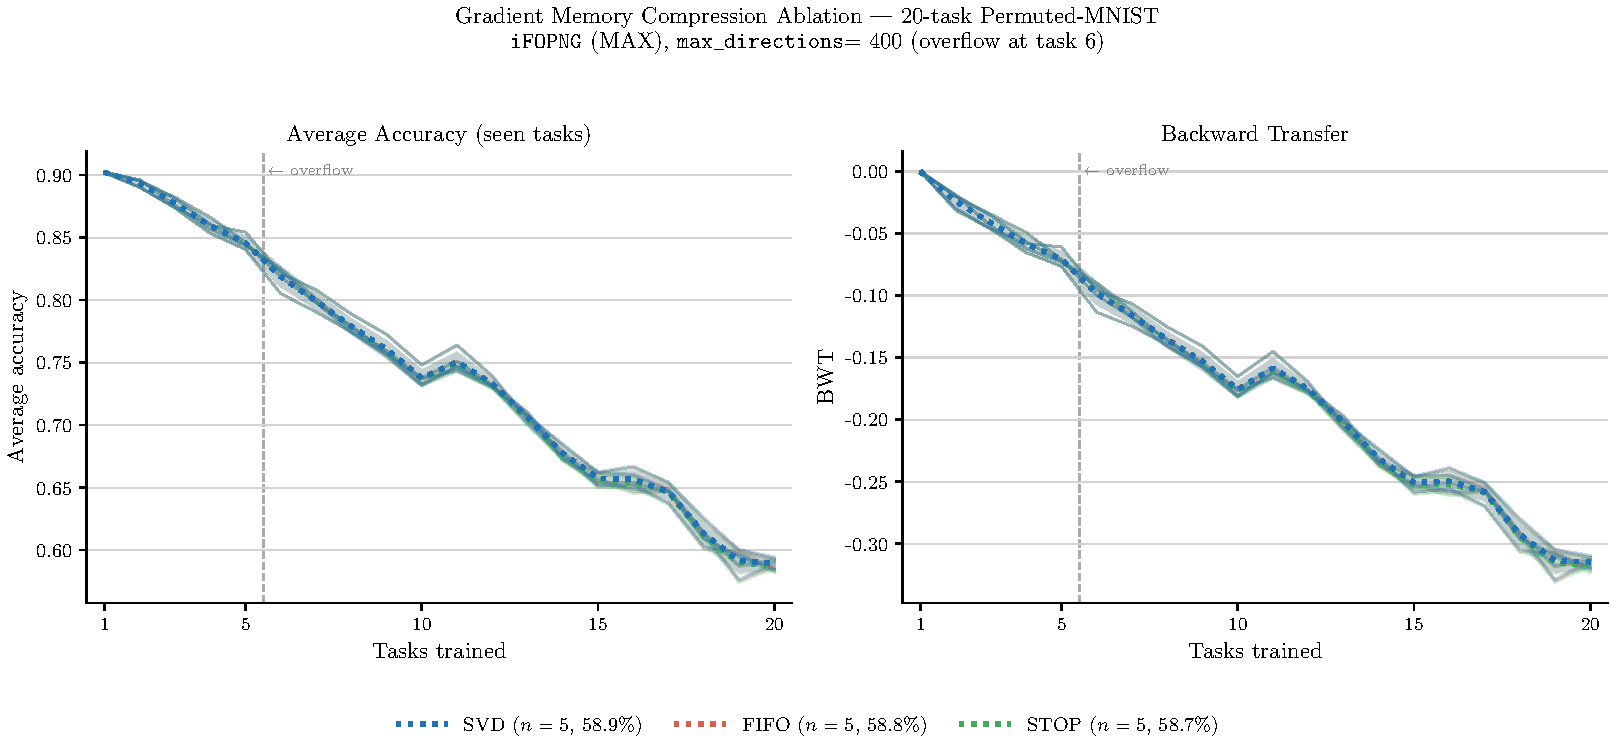
\includegraphics[width=\linewidth]{figures/compression-ablation_421-422-423.pdf}
\caption{%
        \textbf{Gradient memory compression ablation ---
        20-task Permuted-MNIST, \texttt{iFOPNG} with MAX accumulation,
        \texttt{max\_directions}$= 400$, $n = 5$ seeds each.}
        Left: average accuracy trajectory over 20 tasks (thick line =
        seed mean; shaded band = $\pm 1$ standard deviation).
        Right: backward transfer trajectory from task~2 onward.
        The vertical dashed line marks the first compression event at
        task~6, at which point the gradient basis is full and each new
        task's directions displace existing ones according to strategy.
        %
        Three strategies are compared: SVD (retain top-$K$ singular
        vectors), FIFO (evict oldest task directions), and STOP
        (freeze basis, discard new directions).
        All three trajectories are visually indistinguishable throughout;
        final average accuracy spans $58.71\%$--$58.93\%$,
        a between-condition range of $0.22$~pp.
        The result confirms that allocation strategy is dominated by
        budget size: with $400$ directions for 20 tasks
        ($\approx 20$ per task), the binding constraint is the
        budget-to-task ratio rather than how the budget is distributed.
        On Permuted-MNIST, where task distributions are structurally
        homogeneous, all gradient directions carry equal importance and
        SVD's importance-weighted selection provides no measurable
        advantage over the simpler alternatives.
    }
\label{fig:compression_ablation}
\end{figure}


% ── D.6  Seed-2137 initialization failure — Split-MNIST HN ──────────────────

\begin{figure}[H]
\centering
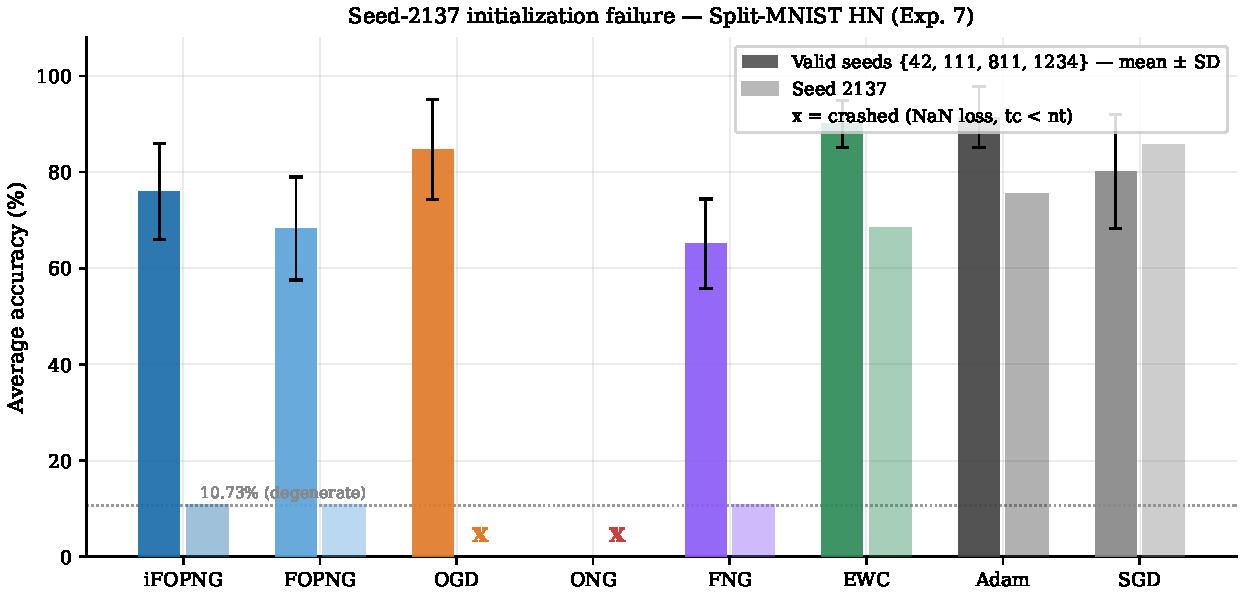
\includegraphics[width=\linewidth]{figures/seed2137_failure_exp7.pdf}
\caption{%
    \textbf{Seed-2137 initialization failure --- Split-MNIST hypernetwork
    ($d_h = 8$, 5 tasks, task-incremental single-head).}
    Each group of bars shows average accuracy for one method; within each
    group the lighter bar is the mean over the four valid seeds
    $\{42, 111, 811, 1234\}$ ($\pm 1$ SD, shown as error bar) and the darker
    bar is the value obtained under seed~2137.
    Methods whose seed-2137 bar is absent (\texttt{OGD}, \texttt{ONG})
    crashed with \texttt{NaN} train loss at task~1 and produced no
    evaluable result.
    %
    The failure is selective by method class.
    Unconstrained baselines (\texttt{Adam}, \texttt{SGD}) and
    \texttt{EWC} show no anomaly under seed~2137, converging normally and
    posting results within the valid-seed distribution.
    Every gradient-memory method (\texttt{FNG}, \texttt{FOPNG},
    \texttt{iFOPNG}) converges to an identical degenerate accuracy of
    $10.73\%$ --- a value equal to the single-task mean across the five
    tasks, indicating that task~1 was learned normally
    ($53.7\%$ of final accuracy attributable to task~1 alone) while
    every subsequent task was never learned.
    %
    The underlying mechanism is a shared task-1 initialization failure.
    Under this seed, all adaptive-optimizer runs of the hypernetwork
    converge to a degenerate task-1 solution at $53.7\%$ accuracy
    (barely above binary chance on the 5-task single-head protocol)
    rather than the $\approx 99\%$ reached by SGD on the same seed.
    Methods that carry nothing forward from task~1 (Adam, EWC) recover
    by learning tasks 2--5 independently.
    Methods that bootstrap their gradient memory $G$ and Fisher estimate
    $\hat{F}$ from the task-1 solution are permanently foreclosed:
    the projection subspace is seeded from a near-random initialisation,
    causing all subsequent gradient updates to be projected to near-zero.
    \texttt{OGD} and \texttt{ONG} additionally overflow during Fisher
    estimation on the untrained task-2 embedding, producing \texttt{NaN}
    propagation consistent with the diagnostic in the thesis body.
    Because the failure is caused by the initialization and affects all
    projection-based methods identically, it renders any cross-method
    comparison on this seed invalid; seed~2137 was therefore replaced by
    seed~314 for the Split-MNIST hypernetwork experiment
    (see Section~\ref{sec:hparam_provenance}).
}
\label{fig:seed2137_failure}
\end{figure}